\documentclass[tikz,border=2mm]{standalone}
\usetikzlibrary{patterns}
\begin{document}
	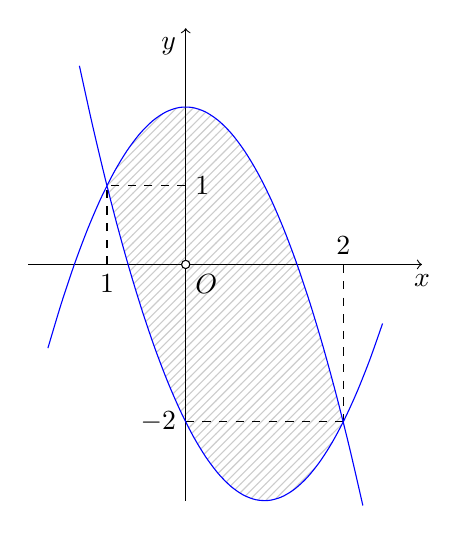
\begin{tikzpicture}[declare function={
			f(\x)=(\x)^2-2*(\x)-2;
			g(\x)=-(\x)^2+2;
		}]
		\path[pattern=north east lines,pattern color=gray!40] plot[domain=-1:2] (\x,{f(\x)})--
		plot[domain=2:-1] (\x,{g(\x)})--cycle;
		\draw[dashed]
		(-1,0) node[below]{$1$}--(-1,1)
		(0,1) node[right]{$1$}--(-1,1)
		(2,0) node[above]{$2$}--(2,-2)
		(0,-2) node[left]{$-2$}--(2,-2);
		\draw[->] (-2,0)--(3,0) node[below]{$x$};
		\draw[->] (0,-3)--(0,3) node[below left]{$y$};
		\draw[fill=white] (0,0) circle(1.5pt) node[below right]{$O$};
		\draw[blue,smooth]
		plot[domain=-1.35:2.5] (\x,{f(\x)})
		plot[domain=-1.75:2.25](\x,{g(\x)});
	\end{tikzpicture}
\end{document}